\documentclass[a4paper, 12pt]{article}
\usepackage[utf8]{inputenc}
\usepackage[russian,english]{babel}
\usepackage[T2A]{fontenc}
\usepackage[left=10mm, top=20mm, right=10mm, bottom=15mm, footskip=13mm]{geometry}
\usepackage{indentfirst}
\usepackage{amsmath,amssymb}
\usepackage{graphicx}
\usepackage[italicdiff]{physics}
\usepackage{float}
\usepackage{array}
\usepackage{physics}
\graphicspath{ {shema/} {graphic/} }
\usepackage{caption}
\captionsetup[figure]{name=Рисунок}
  
\title{Отчет по лабораторной работе 1.3.1

Определение модуля Юнга на основе исследования деформаций растяжения и изгиба}

\author{Максим Осипов, Б03-504}
\date{01.10.2025}

\begin{document}
\maketitle
\newpage
\section{Аннотация}
В данной лабораторной работе экспериментально исследуется зависимость между напряжением и деформацией для упругих тел с целью определения модуля Юнга. Работа состоит из двух частей. В первой части изучается деформация одноосного растяжения проволоки с использованием прибора Лермантова, где удлинение измеряется по углу поворота зеркальца. Во второй части исследуется деформация чистого изгиба балки, опирающейся на две призмы. Модуль Юнга определяется по величине прогиба её середины под действием известной нагрузки, приложенной в центре. Для расчёта используются измеренные геометрические параметры стержня и расстояние между опорами.

\section{Теоретическая справка}
\subsection{Определение модуля Юнга по измерениям растяжения проволоки}


Для определения модуля Юнга по измерениям растяжения используется прибор Лермантова. Верхний конец проволоки прикреплен к консоли, а нижний - к цилиндру шарнирного кронштейна. На этот цилиндр опирается рычаг, связанный с зеркальцем, что позволяет измерять удлинение проволоки по углу поворота зеркальца.

\begin{figure}[h]
\centering
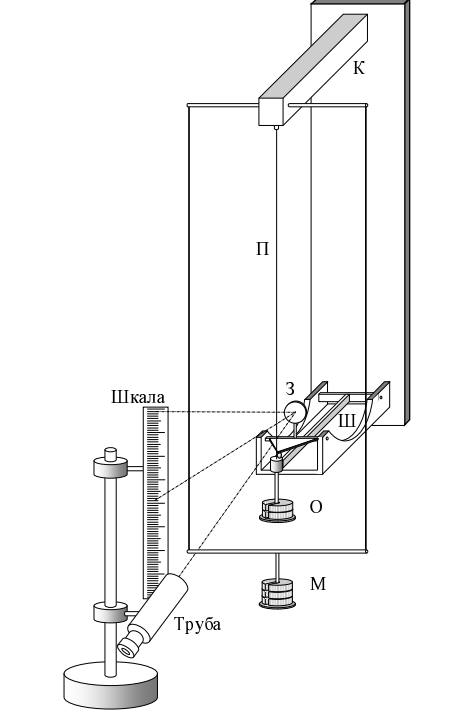
\includegraphics[width=0.4\linewidth]{прибор Лермантова.png}
\caption{Прибор Лермантова }
\label{fig:voltage_current}
\end{figure}

\newpage

\subsection{Определение модуля Юнга по измерениям изгиба}
Для определения модуля Юнга по измерениям изгиба используется установка, состоящая из прочной стойки с опорными призмами A и B. На ребра призм опирается исследуемый стержень. В середине стержня на призме подвешена площадка с грузами. Стрелу прогиба измеряют с помощью индикатора.

\begin{figure}[h]
\centering
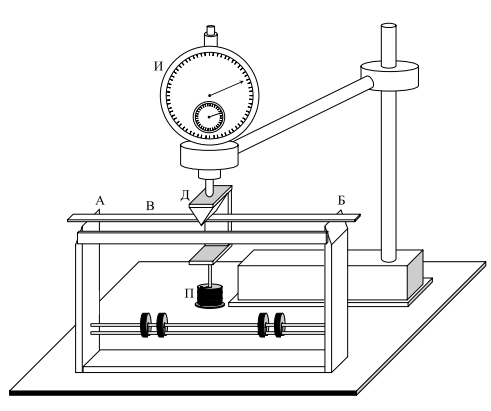
\includegraphics[width=0.5\linewidth]{схема установки.png}
\caption{Схема установки}
\label{fig:voltage_current}
\end{figure}

Модуль Юнга E материала стержня связан со стрелой прогиба y_max соотношением:

\[ E = \frac{P l^3}{4ab^3 y_{\max}} \]
где P - нагрузка, вызывающая прогиб стержня, l - расстояние между призмами A и B, a и b - ширина и высота сечения стержня.














\end{document}